% fig7_19.tex — 7-21: 弹簧 + 平板 + 两个圆柱纯滚动
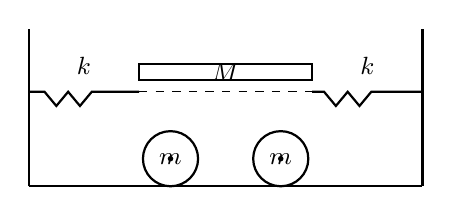
\begin{tikzpicture}[font=\small,>=stealth]
  % 地面
  \draw[thick] (-2.5,-1.2) -- (2.5,-1.2);
  % 左墙
  \draw[thick] (-2.5,-1.2) -- (-2.5,0.8);
  % 右墙
  \draw[thick] (2.5,-1.2) -- (2.5,0.8);
  % 左弹簧 k
  \draw[thick] (-2.5,0) -- ++(0.2,0)
    foreach \i in {1,...,4}{
      -- ++(0.15,{(-1)^\i*0.18})
    } -- (-1.1,0);
  % 右弹簧 k
  \draw[thick] (1.1,0) -- ++(0.15,0)
    foreach \i in {1,...,4}{
      -- ++(0.15,{(-1)^\i*0.18})
    } -- (2.5,0);
  % 平板 M
  \draw[thick,fill=white] (-1.1,0.15) rectangle (1.1,0.35);
  \node at (0,0.25) {$M$};
  % 左圆柱 m
  \draw[thick] (-0.7,-0.85) circle (0.35);
  \fill (-0.7,-0.85) circle (1pt);
  \node at (-0.7,-0.85) {$m$};
  % 右圆柱 m
  \draw[thick] (0.7,-0.85) circle (0.35);
  \fill (0.7,-0.85) circle (1pt);
  \node at (0.7,-0.85) {$m$};
  % 圆柱接触线
  \draw[dashed] (-1.1,0) -- (1.1,0);
  % 标注
  \node[above] at (-1.8,0.1) {$k$};
  \node[above] at (1.8,0.1) {$k$};
\end{tikzpicture}
